%%%%%%%%%%%%%%%%%%%%%%%%%%%%%%%%%%%%%%%%%
% Programming/Coding Assignment
% LaTeX Template
%
% This template has been downloaded from:
% http://www.latextemplates.com
%
% Original author:
% Ted Pavlic (http://www.tedpavlic.com)
%
% Note:
% The \lipsum[#] commands throughout this template generate dummy text
% to fill the template out. These commands should all be removed when 
% writing assignment content.
%
% This template uses a Perl script as an example snippet of code, most other
% languages are also usable. Configure them in the "CODE INCLUSION 
% CONFIGURATION" section.
%
%%%%%%%%%%%%%%%%%%%%%%%%%%%%%%%%%%%%%%%%%

%----------------------------------------------------------------------------------------
%	PACKAGES AND OTHER DOCUMENT CONFIGURATIONS
%----------------------------------------------------------------------------------------



\documentclass{article}

\usepackage{fancyhdr} % Required for custom headers
\usepackage{lastpage} % Required to determine the last page for the footer
\usepackage{extramarks} % Required for headers and footers
\usepackage[usenames,dvipsnames]{color} % Required for custom colors
\usepackage{graphicx} % Required to insert images
\usepackage{listings} % Required for insertion of code
\usepackage{courier} % Required for the courier font

\usepackage[linesnumbered,algoruled,boxed,lined]{algorithm2e}
\usepackage[noend]{algpseudocode}
\usepackage{amsmath}
\usepackage{amssymb}
% Margins
\topmargin=-0.45in
\evensidemargin=0in
\oddsidemargin=0in
\textwidth=6.5in
\textheight=9.0in
\headsep=0.25in

\linespread{1.1} % Line spacing

% Set up the header and footer
\pagestyle{fancy}
\lhead{\hmwkAuthorName} % Top left header
\chead{\hmwkClass\ (\hmwkClassInstructor\ \hmwkClassTime): \hmwkTitle} % Top center head
\rhead{\firstxmark} % Top right heaer
\lfoot{\lastxmark} % Bottom left footer
\cfoot{} % Bottom center footer
\rfoot{Page\ \thepage\ of\ \protect\pageref{LastPage}} % Bottom right footer
\renewcommand\headrulewidth{0.4pt} % Size of the header rule
\renewcommand\footrulewidth{0.4pt} % Size of the footer rule

\setlength\parindent{0pt} % Removes all indentation from paragraphs

%----------------------------------------------------------------------------------------
%	CODE INCLUSION CONFIGURATION
%----------------------------------------------------------------------------------------

\definecolor{MyDarkGreen}{rgb}{0.0,0.4,0.0} % This is the color used for comments
\lstloadlanguages{python} % Load Perl syntax for listings, for a list of other languages supported see: ftp://ftp.tex.ac.uk/tex-archive/macros/latex/contrib/listings/listings.pdf
\lstset{language=Perl, % Use Perl in this example
        frame=single, % Single frame around code
        basicstyle=\small\ttfamily, % Use small true type font
        keywordstyle=[1]\color{Blue}\bf, % Perl functions bold and blue
        keywordstyle=[2]\color{Purple}, % Perl function arguments purple
        keywordstyle=[3]\color{Blue}\underbar, % Custom functions underlined and blue
        identifierstyle=, % Nothing special about identifiers                                         
        commentstyle=\usefont{T1}{pcr}{m}{sl}\color{MyDarkGreen}\small, % Comments small dark green courier font
        stringstyle=\color{Purple}, % Strings are purple
        showstringspaces=false, % Don't put marks in string spaces
        tabsize=5, % 5 spaces per tab
        %
        % Put standard Perl functions not included in the default language here
        morekeywords={rand},
        %
        % Put Perl function parameters here
        morekeywords=[2]{on, off, interp},
        %
        % Put user defined functions here
        morekeywords=[3]{test},
       	%
        morecomment=[l][\color{Blue}]{...}, % Line continuation (...) like blue comment
        numbers=left, % Line numbers on left
        firstnumber=1, % Line numbers start with line 1
        numberstyle=\tiny\color{Blue}, % Line numbers are blue and small
        stepnumber=5 % Line numbers go in steps of 5
}

% Creates a new command to include a perl script, the first parameter is the filename of the script (without .pl), the second parameter is the caption
\newcommand{\pythonscript}[2]{
\begin{itemize}
\item[]\lstinputlisting[caption=#2,label=#1]{#1.py}
\end{itemize}
}

%----------------------------------------------------------------------------------------
%	DOCUMENT STRUCTURE COMMANDS
%	Skip this unless you know what you're doing
%----------------------------------------------------------------------------------------

% Header and footer for when a page split occurs within a problem environment
\newcommand{\enterProblemHeader}[1]{
\nobreak\extramarks{#1}{#1 continued on next page\ldots}\nobreak
\nobreak\extramarks{#1 (continued)}{#1 continued on next page\ldots}\nobreak
}

% Header and footer for when a page split occurs between problem environments
\newcommand{\exitProblemHeader}[1]{
\nobreak\extramarks{#1 (continued)}{#1 continued on next page\ldots}\nobreak
\nobreak\extramarks{#1}{}\nobreak
}

\setcounter{secnumdepth}{0} % Removes default section numbers
\newcounter{homeworkProblemCounter} % Creates a counter to keep track of the number of problems

\newcommand{\homeworkProblemName}{}
\newenvironment{homeworkProblem}[1][Problem \arabic{homeworkProblemCounter}]{ % Makes a new environment called homeworkProblem which takes 1 argument (custom name) but the default is "Problem #"
\stepcounter{homeworkProblemCounter} % Increase counter for number of problems
\renewcommand{\homeworkProblemName}{#1} % Assign \homeworkProblemName the name of the problem
\section{\homeworkProblemName} % Make a section in the document with the custom problem count
\enterProblemHeader{\homeworkProblemName} % Header and footer within the environment
}{
\exitProblemHeader{\homeworkProblemName} % Header and footer after the environment
}

\newcommand{\problemAnswer}[1]{ % Defines the problem answer command with the content as the only argument
\noindent\framebox[\columnwidth][c]{\begin{minipage}{0.98\columnwidth}#1\end{minipage}} % Makes the box around the problem answer and puts the content inside
}

\newcommand{\homeworkSectionName}{}
\newenvironment{homeworkSection}[1]{ % New environment for sections within homework problems, takes 1 argument - the name of the section
\renewcommand{\homeworkSectionName}{#1} % Assign \homeworkSectionName to the name of the section from the environment argument
\subsection{\homeworkSectionName} % Make a subsection with the custom name of the subsection
\enterProblemHeader{\homeworkProblemName\ [\homeworkSectionName]} % Header and footer within the environment
}{
\enterProblemHeader{\homeworkProblemName} % Header and footer after the environment
}

%----------------------------------------------------------------------------------------
%	NAME AND CLASS SECTION
%----------------------------------------------------------------------------------------

\newcommand{\hmwkTitle}{Project\ \#2} % Assignment title
\newcommand{\hmwkDueDate}{Wednesday,\ Dec\ 2,\ 2015} % Due date
\newcommand{\hmwkClass}{ CAP 5638} % Course/class
\newcommand{\hmwkClassTime}{10:10am} % Class/lecture time
\newcommand{\hmwkClassInstructor}{XiuWen Liu} % Teacher/lecturer
\newcommand{\hmwkAuthorName}{YongQing Zheng} % Your name

%----------------------------------------------------------------------------------------
%	TITLE PAGE
%----------------------------------------------------------------------------------------

\title{
\vspace{2in}
\textmd{\textbf{\hmwkClass:\ \hmwkTitle}}\\
\normalsize\vspace{0.1in}\small{Due\ on\ \hmwkDueDate}\\
\vspace{0.1in}\large{\textit{\hmwkClassInstructor\ \hmwkClassTime}}
\vspace{3in}
}

\author{\textbf{\hmwkAuthorName}}
\date{} % Insert date here if you want it to appear below your name

%----------------------------------------------------------------------------------------

\begin{document}

\maketitle

%----------------------------------------------------------------------------------------
%	TABLE OF CONTENTS
%----------------------------------------------------------------------------------------

%\setcounter{tocdepth}{1} % Uncomment this line if you don't want subsections listed in the ToC

\newpage
\tableofcontents
\newpage

%%----------------------------------------------------------------------------------------
%%Algorithm test 
%%----------------------------------------------------------------------------------------
%\begin{algorithm}[H]
%Fixed Increment Single Sample Perceptron($a,k,n$)\;
% $a,k\gets 0$\;
%\While{all pattern does not properly classified}{
%$k\gets (k+1)$ mod $n$\;
%\If{$y^k$ is misclassified by $a$}{
%$a\gets a+y^k$\;}
%}
%Return $a$\;
%\caption{Fixed Increment Single Sample Perceptron}
%\end{algorithm}
%
%
%\begin{algorithm}[H]
%\caption{Batch relaxation with Margin}\label{alg:2}
%\SetKwInOut{Keyword}{Keyword}
%Batch Relaxation with Margin($a,\eta (.),b,k$)\;
%$a,\eta (.),b,k\gets 0$\;
%
%\While{$y^k \neq \{\}$}
%{
%$k\gets (k+1)$ mod $n$\;
%$y^k=\{\}$\;
%$j=0$\;
%\While{$j \neq n$}
%{
%$j \gets j+1$\;
%\If{$a^ty^j\leq b$} 
%{Append $y^j$ to $y^k$\;
%}
%}
%$a\gets a+\eta(k)\sum_{y\in y}\frac{b-a^ty}{||y||^2}y$\;
%}
%\textbf{Return} $a$
%\end{algorithm}
%
%
%\begin{algorithm}[H]
%\caption{Adaboost}\label{alg:3}
%Adaboost\;
%$D=\{x_1,y^1,...,x^n,y_n$\},$k_{max}$,$W_1(i)=1/n,i=1,...,n$\;
%$k\gets 0$\;
%\While{$k\leq k_{max}$}
%{
%train weak learner $C_k$ using $D$ sampled according to $W_k(i)$\;
%$E_k \gets$ training error of $C_k$ measured on $D$ using $W_k(i)$\;
%$\alpha_k \gets \frac{1}{2}ln[(1-E_k)/E_k)]$\;
%\begin{equation*}
%W_{k+1}(i)\gets \frac{W_k(i)}{Z_k}\prod \left\{
%\begin{aligned}
%&e^{-\alpha_k} & & if\ h_k(x^i)=y_i\ (correctly\ classified)\\
%&e^{\alpha_k} & & if\ h_k(x^i)\neq y_i\ (incorrectly\ classified)
%\end{aligned}
%\right. 
%\end{equation*}
%}
%Return $C_k$ and $\alpha_k$ for $k=1$ to $k_{max}$ (ensemble of classifiers with weights)\;
%\end{algorithm}
%------------------------------------
% % algorithm2e include function 
%------------------------------------
%\documentclass{article}
%\usepackage[vlined,ruled]{algorithm2e}
%\usepackage{xcolor}
%
%%%% optional fonts and color configuration
%\SetAlFnt{\sffamily}
%\renewcommand\ArgSty{\normalfont\sffamily}
%\renewcommand\KwSty[1]{\textnormal{\textbf{\sffamily#1}}\unskip}
%\SetAlCapFnt{\normalfont\sffamily\large}
%\renewcommand\AlCapNameFnt{\sffamily\large}
%
%%%% vertical rules in cyan color
%\makeatletter
%\renewcommand{\algocf@Vline}[1]{%     no vskip in between boxes but a strut to separate them, 
%  \strut\par\nointerlineskip% then interblock space stay the same whatever is inside it
%  \algocf@push{\skiprule}%        move to the right before the vertical rule
%  \hbox{\bgroup\color{cyan}\vrule\egroup%
%    \vtop{\algocf@push{\skiptext}%move the right after the rule
%      \vtop{\algocf@addskiptotal #1}\bgroup\color{cyan}\Hlne\egroup}}\vskip\skiphlne% inside the block
%  \algocf@pop{\skiprule}%\algocf@subskiptotal% restore indentation
%  \nointerlineskip}% no vskip after
%%
%\renewcommand{\algocf@Vsline}[1]{%    no vskip in between boxes but a strut to separate them, 
%  \strut\par\nointerlineskip% then interblock space stay the same whatever is inside it
%  \algocf@bblockcode%
%  \algocf@push{\skiprule}%        move to the right before the vertical rule
%  \hbox{\bgroup\color{cyan}\vrule\egroup%               the vertical rule
%    \vtop{\algocf@push{\skiptext}%move the right after the rule
%      \vtop{\algocf@addskiptotal #1}}}% inside the block
%  \algocf@pop{\skiprule}% restore indentation
%  \algocf@eblockcode%
%}
%%
%\makeatother
%%%% end of optional fonts and color configuration
%
%\SetKwProg{Fn}{Function}{}{}
%
%\begin{document}
%
%\begin{algorithm}
%\Fn{BuildOLD (directory)}{
% enter directory\;
% geometrylist $\leftarrow$ search geometry files\;
% $np$ $\leftarrow$ number of total processes\;
% $ng$ $\leftarrow$ number of total geometry files\;
% \eIf{$ng < np$ and $processid < ng$}{
%   GenSeparateLODFile(geometrylist[processid])\;
%   }{
%   sort geometrylist by file size\;
%   \While{i*processid $<$ ng}{
%        GenSeparateLODFile(geometrylist[processid*i])\;
%        $i$++\;
%    }
%  }
%  wait for all processes to end\;
%    \If{isLastProcess}{
%        assembly each LOD geometry\;
%    }}
%\caption{PLG}
%\end{algorithm}
%
%\end{document}
%-----------------------------------------------
%Add program
%-----------------------------------------------


%\begin{homeworkProblem}
%Listing \ref{assignment} shows a python script.
%
%\pythonscript{assignment}{Python program for the project}
%
%\lipsum[1]
%\end{homeworkProblem}


%-----------------------------
%start the project
%-----------------------------

\begin{homeworkProblem}

\textbf{\Large{[Background:]}}\\

Bayesian decision theory provides the optimal decision rule for classification when the true probabilities are known. However, for pattern classification applications, the final product we need is a classifier which can be represented by a set of discriminant function. Therefore, if we can learn discriminant functions directly, we can avoid the intermediate step of estimating probability models,which arguably is more difficult than learning discriminant functions with finite training data(note that by doing this we lose the first principle and many techniques are thus ad hoc).
Linear discriminant functions are widely used because they are efficient and can often be analyzed analytically. Besides, through kernel methods and boosting algorithms, they can lead to accurate classifiers for complex, real-world applications.\\

\textbf{\Large{[Purpose:]}}\\

Learn how to realize the two class/multi-class linear discriminant functions through perceptron-like algorithms and how to use boosting algorithms to build more accurate classifiers using linear discriminant functions.\\
Learn how to use the two class classification algorithm to deal with the multi-class classification problem.\\
 
\textbf{\Large{[Methodology:]}}\\

Implement Algorithm 4(Fixed-increment Single-sample Perceptron Algorithm) and Algorithm 8 (Batch Relaxation with Margin) of chapter 5 as the basic classifiers. Use boost method Algorithm 8 (Adaboost) to create a strong classifier based on the weak classifier. The description of the three algorithm are as follows:\\


\IncMargin{1ex}
\begin{algorithm}
Fixed Increment Single Sample Perceptron($a,k,n$)\;
 $a,k\gets 0$\;
\While{all pattern does not properly classified}{
$k\gets (k+1)$ mod $n$\;
\If{$y^k$ is misclassified by $a$}{
$a\gets a+y^k$\;}
}
Return $a$\;
\caption{Fixed Increment Single Sample Perceptron}
\end{algorithm}

\IncMargin{1ex}
\begin{algorithm}
\caption{Batch relaxation with Margin}\label{alg:2}
\SetKwInOut{Keyword}{Keyword}
Batch Relaxation with Margin($a,\eta (.),b,k$)\;
$a,\eta (.),b,k\gets 0$\;

\While{$y^k \neq \{\}$}
{
$k\gets (k+1)$ mod $n$\;
$y^k=\{\}$\;
$j=0$\;
\While{$j \neq n$}
{
$j \gets j+1$\;
\If{$a^ty^j\leq b$} 
{Append $y^j$ to $y^k$\;
}
}
$a\gets a+\eta(k)\sum_{y\in y}\frac{b-a^ty}{||y||^2}y$\;
}
\textbf{Return} $a$
\end{algorithm}

\vspace{2ex}
\begin{algorithm}[H]
\caption{Adaboost}\label{alg:3}
Adaboost\;
$D=\{x_1,y^1,...,x^n,y_n$\},$k_{max}$,$W_1(i)=1/n,i=1,...,n$\;
$k\gets 0$\;
\While{$k\leq k_{max}$}
{
train weak learner $C_k$ using $D$ sampled according to $W_k(i)$\;
$E_k \gets$ training error of $C_k$ measured on $D$ using $W_k(i)$\;
$\alpha_k \gets \frac{1}{2}ln[(1-E_k)/E_k)]$\;
\begin{equation*}
W_{k+1}(i)\gets \frac{W_k(i)}{Z_k}\prod \left\{
\begin{aligned}
&e^{-\alpha_k} & & if\ h_k(x^i)=y_i\ (correctly\ classified)\\
&e^{\alpha_k} & & if\ h_k(x^i)\neq y_i\ (incorrectly\ classified)
\end{aligned}
\right. 
\end{equation*}
}
Return $C_k$ and $\alpha_k$ for $k=1$ to $k_{max}$ (ensemble of classifiers with weights)\;
\end{algorithm}

To deal with the multi-class classification problem, we use the one against other and one against rest methods. For the one against rest method, we need to build $p$ classifiers based on one class against the rest, and choose the final class which has the maximum linear discriminant function result. For the one against other method, we need to build $p(p-1)/2$ classifiers based on the each pairs of the class and use the voting scheme to decide the class of the test data.\\

\textbf{\Large{[Dataset:]}}\\

We use two dataset to build and test our model.\\
The first one is UCI wine dataset. Training set of this data consists of 89 examples in three class(30 in class 1, 36 in class 2 and 24 in class 3). The test set consists also of 89 examples(29 in class 1, 36 in class 2, and 24 in class 3). \\
Another is USPS handwritten digit dataset. The training set consists of 2930 training samples (1194 in digit 0,1005 in digit 1, and 731 in digit 2). The test set consists of 821 samples(359 in digit 0, 264 in digit 1 and 198 in digit 2)\\


\textbf{\Large{[Expriment results:]}}\\

We use Matlab and python to build our model to solve this project. From our calculation, we found that the USPS dataset was linearly separable compared with the UCI dataset which might not be properly separated. 
\begin{figure}[htb!]
  \caption{Analysis of the UCI data set}
    \centering
    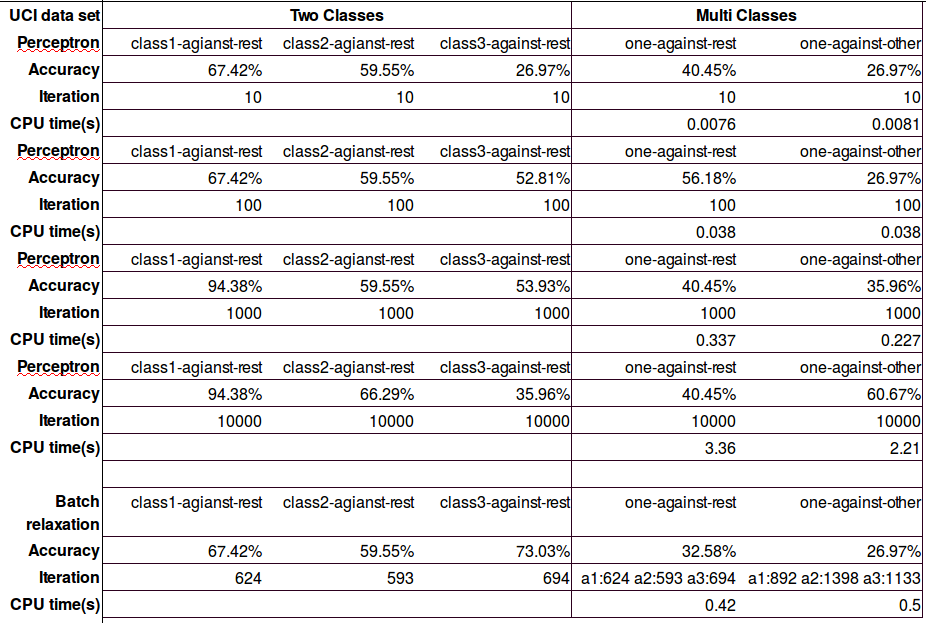
\includegraphics[scale =0.5]{uci.png}
\end{figure}

Figure 1 shows the result of both two class and multi-class problem. For each problem, we use two algorithm, Perceptron and Batch relaxation methods, to predict the class based on UCI data training and testing set. The Perceptron algorithm for this data set does not converge, since we can see that when the iteration numbers increases(x10), the accuracy rate does not change a lot, sometimes even decreases.
For the perceptron method, it performances better for the class 1 against rest situation compared with other two cases. For the Batch relaxation method, we use $\eta$ equal to 0.1 and b equal to 1. It converge for the training data, the iteration number is around 600. Class 3 against rest works better for this classifier. \\

\begin{figure}[H]
  \caption{Analysis of the USPS data set}
    \centering
    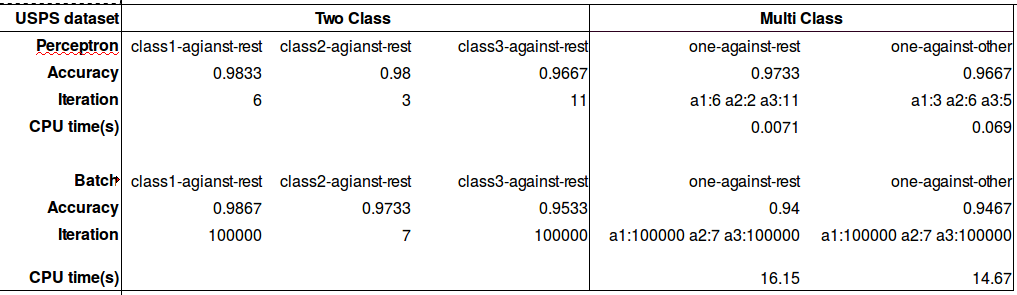
\includegraphics[scale =0.5]{usps.png}
\end{figure}


From Figure 2, we can see that both perceptron and batch relaxation performance excellent on the USPS data set.The accuracy rate for all the two classes cases are above 95\%, besides, for the multi-class problem, both the one against and one against other algorithm are efficient. Perceptron method is a little better than Batch relaxation method for the multi-class problem, around 97 \% accuracy rate vs around 94 respectively\%.
\\
Figure 3 to Figure 6 show the result of ada boosting based on the above two weaker classifier. We also consider the UCI and USPS data together.\\
\begin{figure}[H]
  \caption{Results for UCI data without ada boosting}
    \centering
    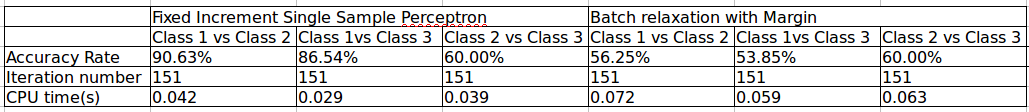
\includegraphics[scale =0.5]{wine_noada.png}
\end{figure}

\begin{figure}[H]
  \caption{Results for UCI data with ada boosting}
    \centering
    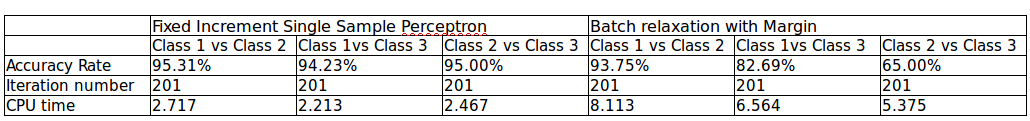
\includegraphics[scale =0.5]{wine_ada.png}
\end{figure}

Figure 3 and figure 4 show the influence of the adaboosting method on the UCI data set, we use both perceptron and batch relaxation methods as weaker classifier. Since the UCI dataset is not linearly separated, we can see from the table, results for both algorithms with boosting performances better than the algorithm without boosting. Let's take Fixed single sample perceptron as example, under the Class 1 vs Class 3 cases, boosting method increase the accuracy rate from 86.54\% to 94.23\%.  \\

\begin{figure}[H]
  \caption{Results for USPS data without ada boosting}
    \centering
    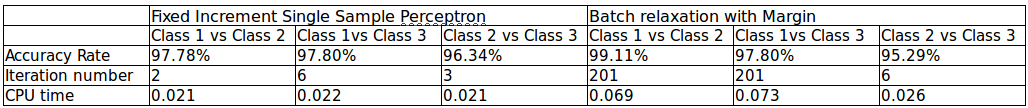
\includegraphics[scale =0.5]{zip_noada.png}
\end{figure}

\begin{figure}[H]
  \caption{Results for USPS data with ada boosting}
    \centering
    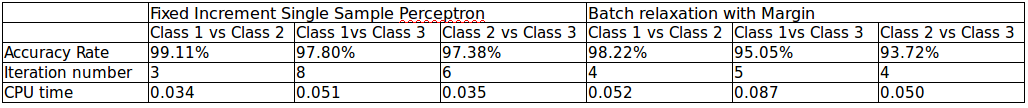
\includegraphics[scale =0.5]{zip_ada.png}
\end{figure}

Figure 5 and Figure 6 gives us the testing predicting results of USPS data based on two algorithms with and without ada-boosting.

Since this dataset is nearly linearly separable, so the original classifier itself can give a very good classification results. According to this reason, methods with boosting does not improve the result significantly. All the results for the one against other methods are above or around 95 \%\\

\textbf{\Large{[Program:]}}\\

Our team use both Matlab and python to realize the programming process for this project. The attachment is the code for reference.\\

List \ref{project2} shows a python and matlab script.

\pythonscript{project2}{Python program for the project}



\end{homeworkProblem}

%\begin{homeworkProblem}
%Problem 1, Chapter 3 of the textbook\\
%Let $x$ have an exponential density:\\
%\begin{equation*}
%p(x|\theta)=\left\{
%\begin{aligned}
%&\theta e^{-\theta x} & & x\geq 0\\
%&0 & & otherwise
%\end{aligned}
%\right. 
%\end{equation*}
%
%(a) Plot $p(x|\theta)$ versus $x$ for $\theta=1$. Plot $p(x|\theta)$ versus $\theta$, ($0\leq \theta \leq 5)$, for $x=2$.\\
%(b) Suppose that $n$ samples $x_1,...,x_n $ are drawn independently according to $p(x|\theta)$.\\
%Show that the maximum likelihood estimate fo $\theta$ is given by:\\
%\begin{equation*}
%\hat{\theta}=\frac{1}{\frac{1}{n}\sum_{k=1}^{n} x_k}\\
%\end{equation*}
%
%Answer:\\
%(a)we draw the chart as follows, the first chart is $p(x|\theta)$ versus $x$ for $\theta=1$ and the second chart is $p(x|\theta)$ versus $\theta$, ($0\leq \theta \leq 5)$, for $x=2$\\
%
%\begin{center}
%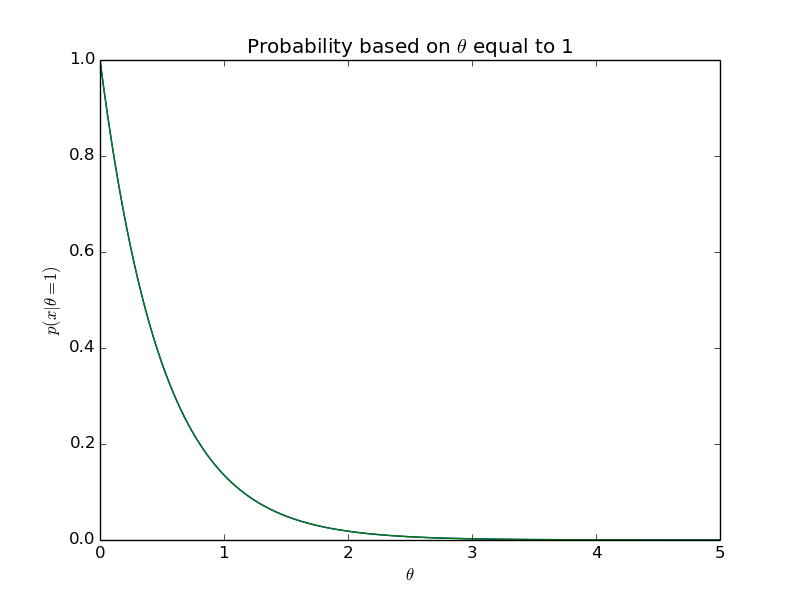
\includegraphics[width=0.75\columnwidth]{prob_theta.png}
%% Example image
%\end{center}
%
%\begin{center}
%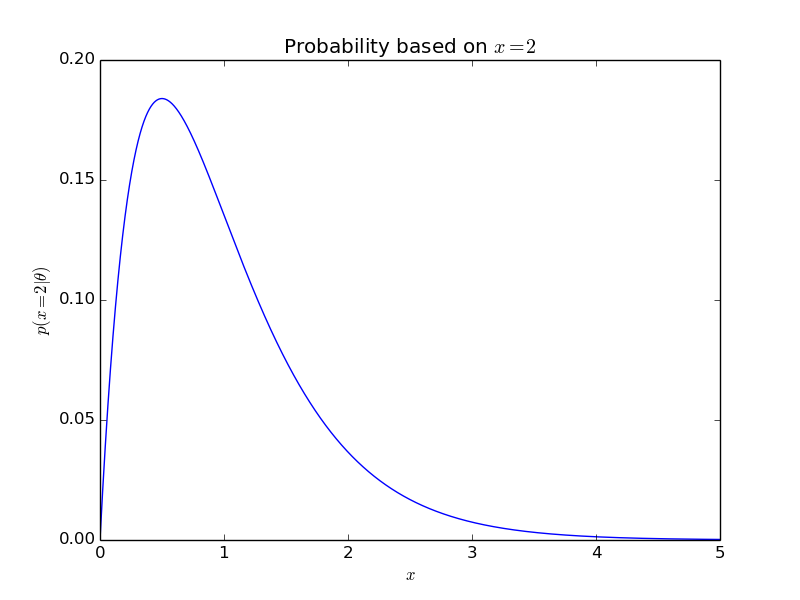
\includegraphics[width=0.75\columnwidth]{prob_x.png}
%% Example image
%\end{center}
%
%(b)The log-likelihood function is:\\
%
%\begin{equation*}
%l(\theta)= \sum_{k=1}^n ln p(x_k|\theta)=\sum_{k=1}^{n}[ln\theta-\theta x_k]=nln\theta - \theta\sum_{k=1}^{n}x_k
%\end{equation*}
%
%To find the maximum of the likelihood function, we take the first derivative of the above equation. The result is as follows:\\
%\begin{equation*}
%\begin{aligned}
%\nabla_\theta l(\theta) & =  \frac{\partial}{\partial\theta}[nln\theta-\theta\sum_{k=1}^{n}x_k]\\
%& = \frac{n}{\theta}-\sum_{k=1}^{n}x_k=0
%\end{aligned}
%\end{equation*}
%
%So the maximum -likelihood solution is:\\
%\begin{equation*}
%\hat{\theta}=\frac{1}{\frac{1}{n}\sum_{k=1}^{n}x_k}.
%\end{equation*}
%
%\end{homeworkProblem}
%
%\begin{homeworkProblem}
%Problem 3, Chapter 3 of the textbook.\\
%Maximum likelihood methods apply to estimates of prior probabilities as well. Let samples be drawn by successive, independent selections of a state of nature $\omega_i$, with unknown probability $P(\omega_i)$. Let $z_{ik}=1$ , if the state of nature for the $kth$ sample is $\omega_i$ and $z_{ik}=0$ otherwise.\\
%
%(a) Show that \\
%
%\begin{equation*}
%P(z_{i1},...,z_{in}|P(\omega_i))=\prod_{k=1}^{n} P(\omega_i)^{z_{ik}}(1-P(\omega_i))^{1-z_{ik}}
%\end{equation*}
%
%
%(b) Show that the maximum likelihood estimate for $P(\omega_i)$ is\\
%
%\begin{equation*}
%\hat{P}(\omega_i)=\frac{1}{n}\sum_{k=1}^{n}z_{ik}.
%\end{equation*}
%Interpret your result in words.\\
%
%Answer:\\
%
%We denote that \\
%\begin{equation*}
%z_{ik}=\left\{
%\begin{aligned}
%&1 & & if\ the\ state\ of\ nature\ for\ the\ k^{th}\ sample\ is\ \omega_i\\
%& 0 & & otherwise
%\end{aligned}
%\right.
%\end{equation*}
%
%(a) The sample are drawn by successive independently selection of a state of nature $\omega_i$ with probability $P(\omega_i)$. We have then :\\
%\begin{equation*}
%Pr[z_{ik}=1|P(\omega_i)]=P(\omega_i)
%\end{equation*}
%
%and:\\
%\begin{equation*}
%Pr[z_{ik}=0|P(\omega_i)]=1-P(\omega_i)
%\end{equation*}
%we can rewrite the above equation as:\\
%
%\begin{equation*}
%Pr[z_{ik}|P(\omega_i)]=[P(\omega_i)]^{z_{ik}}[1-P(\omega_i)]^{1-z_{ik}}
%\end{equation*}
%By the independence of the successive selections, we have :\\
%\begin{eqnarray*}
%P(z_{i1},...,z_{in}|P(\omega_i)) & =&\prod_{k=1}^{n}P(z_{ik}|P(\omega_i))\\
%&=& \prod_{k=1}^{n}[P(\omega_i)]^{z_{ik}}[1-P(\omega_i)]^{1-z_{ik}}
%\end {eqnarray*}
%
%(b) The log-likelihood as a function of $P(\omega_i)$ is:\\
%\begin{eqnarray*}
%l(P(\omega_i)) &=&  lnP(z_{i1},...,z_{in}|P(\omega_i))\\
%&=& ln[\prod_{k=1}^{n}[P(\omega_i)]^{z_{ik}}[1-P(\omega_i)]^{(1-z_{ik})}]\\
%&=& \sum_{k=1}^n [z_{ik}lnP(\omega_i)+(1-z_{ik})ln(1-P(\omega_i))]
%\end{eqnarray*}
%Therefore, the maximum-likelihood values for the $P(\omega_i)$ must satisfy:\\
%\begin{equation*}
%\nabla _{P(\omega_i)}l(P(\omega_i))=\frac{1}{P(\omega_i)}\sum_{k=1}^{n}z_{ik}-\frac{1}{1-P(\omega_i)}\sum_{k=1}^n(1-z_{ik})=0
%\end{equation*}
%We solve this equation and find :
%
%\begin{equation*}
%(1-\hat{P}(\omega_i))\sum_{k=1}^n z_{ik}= \hat{P}(\omega_i)\sum_{k=1}^n (1-z_{ik})
%\end{equation*}
%
%which can be rewritten as:\\
%\begin{equation*}
%\sum_{k=1}^nz_{ik}= \hat{P}(\omega_i)\sum_{k=1}^n z_{ik} + n \hat{P}(\omega_i)-\hat{P}(\omega_i)\sum_{k=1}^n z_{ik}
%\end{equation*}
%
%So the final solution is then:\\
%\begin{equation*}
%\hat{P}(\omega_i)=\frac{1}{n}\sum_{k=1}^n z_{ik}
%\end{equation*}
%
%That is, the estimate of the probability of category $\omega_i$ is merely the probability of obtaining its indicatory value in the training data,  just as we would expected.
%
%\end{homeworkProblem}
%
%\begin{homeworkProblem}
%Problem 7 , Chapter 3 od the textbook\\
%Show that if our model is poor, the maximum likelihood classifier we derive is not the best
%\textendash even among our (poor) model set \textendash by exploring the following example. Suppose we have two equally probable categories (i.e., p($\omega_1$)=P($\omega_2$)=0.5). Further, we know that $p(x|\omega_1)\sim N(0,1)$ but \textit{assume} that $p(x|\omega_2)\sim N(\mu,1)$. (That is, the parameter $\theta$ we seek by maximum likelihood techniques is the mean of the second distribution.) Image however that the \textit{true} underlying distribution is $p(x|\omega_2)\sim N(1,10^6)$.\\
%(a)what is the value of our maximum likelihood estimate $\mu$, in our poor model, given a large amount of data.\\
%(b)  What is the decision boundary arising from this maximum likelihood estimate in the poor model.\\ 
%(c) Ignore for the moment the maximum likelihood approach, and use the methods from chapter 7 to derive the Bayes optimal decision boundary given the \textit{true} underlying distributions \textendash $p(x|\omega_1) \sim N(0,1)$ and $p(x|\omega_2) \sim N(1,10^6)$. be careful to include all portions pf the decision boundary. \\
%(d) Now consider again classifiers based on the (poor) model assumption of $p(x|\omega_2) \sim N(\mu,1 ).$ Using your result immediately above, find a \textit{new} value of $\mu$ that will give lower error than the maximum likelihood classifier. \\
%(e) Discuss these results, with particular attention to the role of knowledge of the underlying model.\\
%Answer:\\
%
%
%\end{homeworkProblem}
%
%\begin{homeworkProblem}
%problem 10, Chapter 3 of the textbook (hint think about the bias and variance.)
%Suppose we employ a novel method for estimating the mean of a data set, $\mathcal{D}={x_1,x_2,...,x_n}$ : we assign the mean to the value of the first point in the set, i.e., $x_1$.\\
%(a) Show that tis method is unbiased. \\
%(b) State why this method is nevertheless highly undesirable.\\
%
%Anwser:\\
%(a)Consider the novel method of estimating the mean of a set of points as taking its first value, which we denote $M= x_1$,\\
%(a) If the expected value of a statistics is equal to the true value, then we call the statistics unbiased. for this case, if we repeat the selection of the first point of a data set we have:\\
%
%\begin{equation*}
%bias = E(M) -\mu=lim_{K\rightarrow\infty}\frac{1}{K}\sum_{k=1}^{K} M(k)-\mu=0; 
%\end{equation*}
%
%Where $M(k)$ is the first point in data set k drawn from the given distribution.\\
%
%(b) While the unusual method for estimating the mean may indeed be biased, it will generally have large variance, and this is an undesirable property. Note that $E[(x_i)-\mu)^2]=\sigma^2$, and the RMS error, $\sigma$, is independent of n.  This undesirable behavior is quite different from that of the measurement of:\\
%\begin{equation*}
%\bar{x} =\frac{1}{n}\sum_{i =1}{n}x_i
%\end{equation*}
%
%where we see:\\
%
%\begin{eqnarray*}
%E[(\bar{x}-\mu)^2] &=& E[(\frac{1}{n}\sum_{i=1}^{n}x_i-\mu)^2]\\
%&=& \frac{1}{n^2}\sum_{i=1}^{n} [E[(x_i-\mu)^2]\\
%&=& \frac{\sigma^2}{n}
%\end{eqnarray*}
%
%Thus the RMS error, $\sigma/\sqrt{n}$, approaches 0 as $1/\sqrt{n}$. Note that there are many superior method for estimating the mean, for instance the sample mean and some other re-sampling method such as "bootstrap" method. 
%
%\end{homeworkProblem}
%
%\begin{homeworkProblem}
%Suppose that the prior distribution of $\theta$ and the parametric form (a uniform distribution) remain the same as in the example given in section 3.5 in the textbook, compute first the Bayesian estimation of $\theta$ and then the estimated class conditional $p(x|D)$ for $D=\{3,9,7\}$. You need to specify the Bayesian estimation and the class conditional fully (i.e., you need to specify the functions with all required constants). Then plot the class conditional form from 0 to 10.\\
%
%Answer:\\
%
%From the example of the textbook, we know that the prior distribution of $\theta$ is a uniform distribution, which listed in the following:\\
%
%\begin{equation*}
%p(x|\theta)\sim U(0, \theta)=\left\{
%\begin{aligned}
%& 1/ \theta & & 0 \leq x \leq 10\\
%& 0 & & otherwise,  \\
%\end{aligned}
%\right.
%\end {equation*}
%
%Similarly with the example in the textbook, we will sue recursive Bayes methods to estimate $\theta$ and the underlying distribution. Before any data arrive, we have $\pagebreak(\theta|\mathcal{D}^0)=p(\theta)=U(0,10)$
%when our first data point $x_1$=3 arrives, we use the equation 54, from the textbook, to get an improved estimate:\\
%\begin{equation*}
%p(\theta|\mathcal{D}^1) \propto p(x|\theta)p(\theta|\mathcal{D}^0)=\left\{
%\begin{aligned}
%& 1/ \theta & & 3 \leq x \leq 10\\
%& 0 & & otherwise,  \\
%\end{aligned}
%\right.
%\end {equation*}
%When the next data point $ x_2 = 9 $ arrives, we have :\\
%\begin{equation*}
%p(\theta|\mathcal{D}^2) \propto p(x|\theta)p(\theta|\mathcal{D}^1)=\left\{
%\begin{aligned}
%& 1/ \theta^2 & & 9 \leq x \leq \theta\\
%& 0 & & otherwise,  \\
%\end{aligned}
%\right.
%\end {equation*}
%
%when the third data point, which is equal to 7, comes, we have:\\
%
%\begin{equation*}
%p(\theta|\mathcal{D}^3) \propto p(x|\theta)p(\theta|\mathcal{D}^2)=\left\{
%\begin{aligned}
%& 1/ \theta^3 & & 9 \leq x \leq 10\\
%& 0 & & otherwise,  \\
%\end{aligned}
%\right.
%\end {equation*}
% 
%
%The general form of the solution is:\\
%\begin{center}
%$p(\theta|\mathcal{D}^n)\propto 1/\theta^n$ for $\max_x[\mathcal{D}^n]\leq \theta\leq 10$.  
%\end{center}
%
%
%To make the above equation become the density function, we also calculate the constant term in all the $p(\theta|\mathcal{D}_i)$, which listed as follows:\\
%
%\begin{equation*}
%p(\theta|\mathcal{D}^1) =\left\{
%\begin{aligned}
%& 1/(ln(10)-ln(3)*1/ \theta & & 9 \leq x \leq 10\\
%& 0 & & otherwise,  \\
%\end{aligned}
%\right.
%\end {equation*}
%
%\begin{equation*}
%p(\theta|\mathcal{D}^2) =\left\{
%\begin{aligned}
%& 1/(1/9-1/10)*1/ \theta^2 & & 9 \leq x \leq 10\\
%& 0 & & otherwise,  \\
%\end{aligned}
%\right.
%\end {equation*}
%
%\begin{equation*}
%p(\theta|\mathcal{D}^3) =\left\{
%\begin{aligned}
%& 1/(1/162-1/200)*1/ \theta^3 & & 9 \leq x \leq 10\\
%& 0 & & otherwise,  \\
%\end{aligned}
%\right.
%\end {equation*}
%We also plot the result for the $p(\theta|\mathcal{D}^i)$ under 4 cases as follows:\\
%
%\begin{center}
%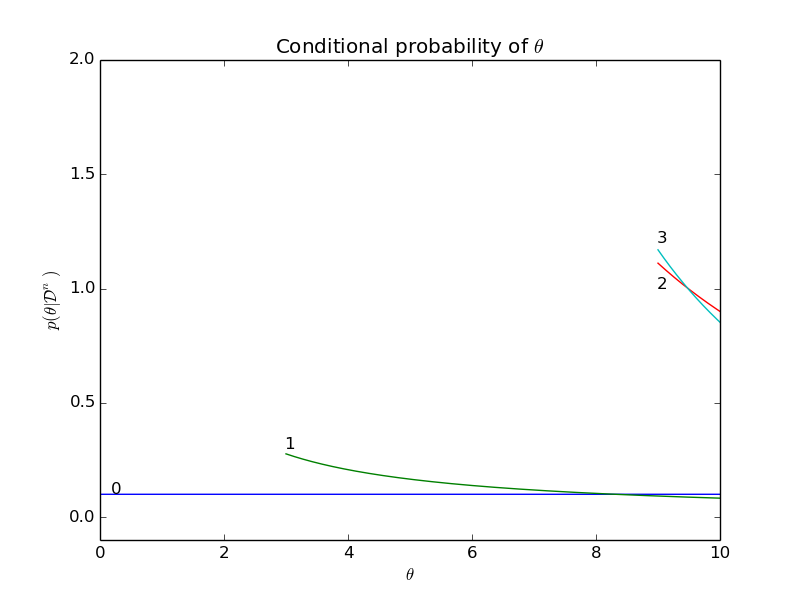
\includegraphics[width=0.75\columnwidth]{conditional_prob_theta.png} % Example image
%\end{center}
%
%next part we try to solve the conditional class probability, $p(x|\mathcal{D}^3)$, given the equation 50 on the text book, we need to solve the integration of the following equation:\\
%\begin{equation*}
%p(x|\mathcal{D})= \int p(x|\theta)p(\theta|\mathcal{D})d\theta 
%\end{equation*}
%note that $\theta$ should be bigger than x and the domain of $\theta$ is 9 to 10 in our case, so in the domain from 0 to 9 of x, the integral region of $\theta$ is 9 to 10, when x bigger than 9, the integral region of $\theta$  becomes x to 10. This means that when x is from 0 to 9, it follows an uniform distribution, and when x is bigger than 9, it follows some polynomial density function. \\ 
%Now we calculate the integration under two situation:\\
%When x is less than 9:\\
%
%\begin{equation*}
%p(x|\mathcal{D})= \int p(x|\theta)p(\theta|\mathcal{D})d\theta =\int_9^{10}
%1/(1/162-1/200)*1/ \theta^4 d\theta=0.10565302144249514
%\end{equation*}
%
%when x is bigger than 9:\\
%
%\begin{equation*}
%p(x|\mathcal{D})= \int p(x|\theta)p(\theta|\mathcal{D})d\theta =\int_x^{10}
%1/(1/162-1/200)*1/ \theta^4 d\theta=1/(1/162-1/200)*1/3*(1/x^3-1/1000)
%\end{equation*}
%
%The following chart shows the result of the conditional class probability in the domain for $x$ from 0 to 10.\\
%
%\begin{center}
%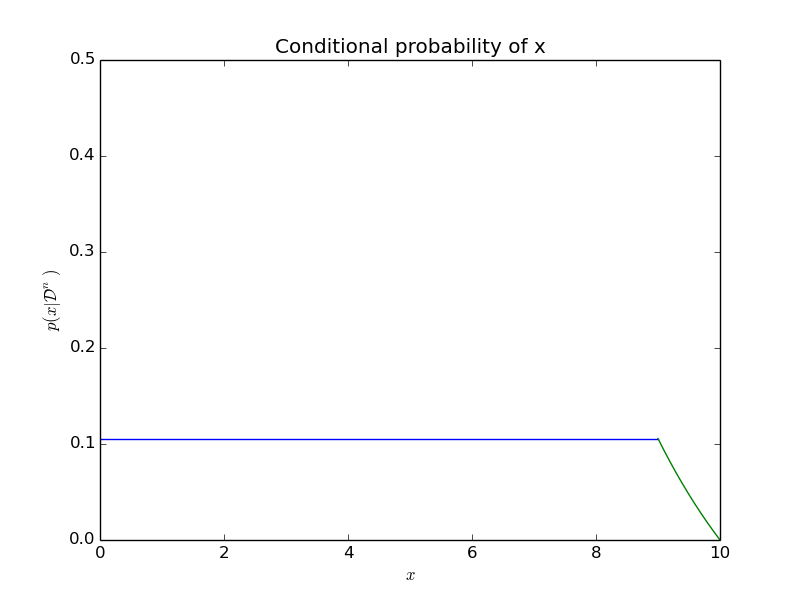
\includegraphics[width=0.75\columnwidth]{conditional_prob_xx.png} % Example image
%\end{center}
%
%\end{homeworkProblem}
%
%\begin{homeworkProblem}
%Problem 11 chapter 3 of the textbook; you only need to show the univariate case.\\
%One measure of the difference between two distribution in the same space is the \textit{Kullback-l=Leibler divergence} of Kullback-Leibler" distance":\\
%\begin{equation*}
%D_{KL}(p_1(x),p_2(x)) = \int {p_1(x)ln\frac{p_1(x)}{p_2(x)}dx}
%\end{equation*}
%( This "distance," does not obey the requisite symmetry and triangle inequalities for a metric.) Suppose we seek to approximate an arbitrary distribution $p_2(x)$ by a normal $p_1(x) \sim N(\mu, \Sigma)$. Show that the values that lead to the smallest Kullback-leibler divergence are the obvious ones:\\
%\begin{equation*}
%\begin{aligned}
%&\mu &=& \mathcal{E}_2[x]\\
%&\Sigma &=& \mathcal{E}_2[(x-\mu)(x-\mu)^t]
%\end{aligned}
%\end{equation*}
%where the expectation taken is over the density $p_(x)$.
%\end{homeworkProblem}

%

%
%
%%----------------------------------------------------------------------------------------
%%	PROBLEM 1
%%----------------------------------------------------------------------------------------
%
%% To have just one problem per page, simply put a \clearpage after each problem
%
%
%\begin{homeworkProblem}
%Listing \ref{homework_example} shows a Perl script.
%
%\perlscript{homework_example}{Sample Perl Script With Highlighting}
%
%\lipsum[1]
%\end{homeworkProblem}
%
%%----------------------------------------------------------------------------------------
%%	PROBLEM 2
%%----------------------------------------------------------------------------------------
%
%\begin{homeworkProblem}
%\lipsum[2]
%
%\problemAnswer{
%\begin{center}
%\includegraphics[width=0.75\columnwidth]{example_figure} % Example image
%\end{center}
%
%\lipsum[3-5]
%}
%\end{homeworkProblem}
%
%%----------------------------------------------------------------------------------------

\end{document}